\section{Establishing the adapter - oscilloscope connection}
    To connect to the oscilloscope to the server, you first need to start the oscilloscope server by setting the oscilloscope listening IP and port on the dashboard (\cref{fig:serv_endp}).

    \begin{figure}[H]
        \begin{center}
        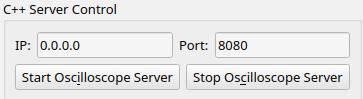
\includegraphics[width = 0.8\textwidth]{img/manual/cserv.png}
        \end{center}
        \caption{Widget to set server endpoint in the oscilloscope}
        \label{fig:serv_endp}
    \end{figure}

    If the server cannot start, a popup will appear with the error.
    
    Once this is done, the adapter can establish a connection to the oscilloscope to send outcome instances (\cref{fig:est_con}). The adapter can now connect to the oscilloscope server.  
    
    \begin{figure}[H]
        \begin{center}
        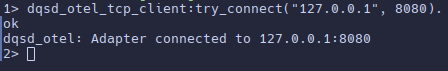
\includegraphics[width = 0.8 \textwidth]{img/manual/connectadapter.png}
        \end{center}
        \caption{Establish connection from adapter to oscilloscope.}
        \label{fig:est_con}
    \end{figure}
    
    We now need to start the listener on the adapter (\cref{fig:est_list}).

     \begin{figure}[H]
        \begin{center}
        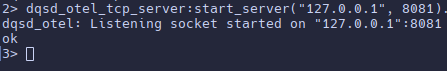
\includegraphics[width = 0.8 \textwidth]{img/manual/listener.png}
        \end{center}
         \caption{Adapter starting listener for commands and parameters from the oscilloscope}.
         \label{fig:est_list}
    \end{figure}

    If an error may arrive during the start-up of the listener, it will be printed out.

    Now, we can connect the oscilloscope to the adapter by setting the listener endpoint (\cref{fig:c_list}).
    
     \begin{figure}[H]
        \begin{center}
        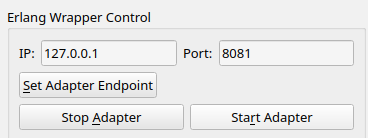
\includegraphics[width = 0.8 \textwidth]{img/manual/endpoint.png}
        \end{center}
         \caption{Set Erlang listener endpoint in oscilloscope.}
         \label{fig:c_list}
    \end{figure}

    If the server cannot connect, an error will pop up. Once connected, the server can start and stop the adapter sending of the spans by clicking the two buttons below.
